% !TEX encoding = UTF-8
% !TEX TS-program = pdflatex
% !TEX root = ../tesi.tex

%**************************************************************
\chapter{Diff \& patch}
\label{cap:diff-patch}
%**************************************************************

Uno degli obiettivi primari del progetto \textit{Stargate} è il supporto prestazionale a grosse mole di dati, dell'ordine di diversi MByte, in continuo aggiornamento ed uso. Finora l'architettura ottimizza il calcolo dello stato derivato all'interno dei \textit{Web Workers} e tutte le operazioni dei widgets attraverso un processo dedicato del Sistema Operativo. \\

Tuttavia entrambe le soluzioni non sono in grado di ottimizzare un potenziale collo-di-bottiglia delle performance: la trasmissione di grosse quantità di dati. Attualmente, ad ogni modifica dello stato applicativo, questi va inviato interamente al \textit{Web Worker} affinché possa calcolare gli stati derivati dei widgets, che a loro volta sono poi inviati ai widgets appunto. \\

Se da un lato tale flusso non abbia impatti negativi sulla pagina principale grazie all'uso di \textit{Web Worker} e processi dedicati, dall'altro potrebbe causare un ritardo nei tempi di aggiornamento dell'Interfaccia Utente nelle finestre widget. Ciò causerebbe una cattiva percezione dell'utente nei confronti della fluidità d'uso dei componenti aperti nelle nuove finestre. \\

D'altra parte è inutilmente dispendioso il continuo invio di tutto lo stato applicativo, che deve essere copiato/serializzato da una parte all'altra. Per tale motivo è stato introdotto un sistema di \textit{diff \& patch} dello stato applicativo.

\section{Flusso diff \& patch}

\begin{enumerate}
  \item All'avvio dell'applicazione, viene inviato lo stato iniziale completo. Per completo si intende che non vi possono essere campi mancati rispetto alla sua interfaccia, sebbene possano avere come valore \texttt{null};
  \item Ad ogni successiva modifica dello stato applicativo, viene calcolata la differenza (ovvero il \textbf{delta $\Delta$}) tra il nuovo stato applicativo e quello precedente. Questa operazione viene chiamata \textbf{diffing};
  \item Il \textit{delta} contiene tutte le informazioni per ricostruire il nuovo stato a partire da quello vecchio. Tale \textit{delta} viene quindi inviato al \textit{Web Worker};
  \item Il \textit{Web Worker} applica il \textit{delta} sullo stato applicativo che ha in memoria, ottenendo il nuovo stato;
  \item Vengono ricalcolati gli stati derivati dei widgets ed un simile processo di \textit{diff \& patch} viene effettuato per essi. Difatti anche i widgets ricevono lo stato derivato intero alla loro apertura, ma i successivi aggiornamenti contengono solo i \textit{delta}.
\end{enumerate}

\begin{figure}[H] 
  \centering 
  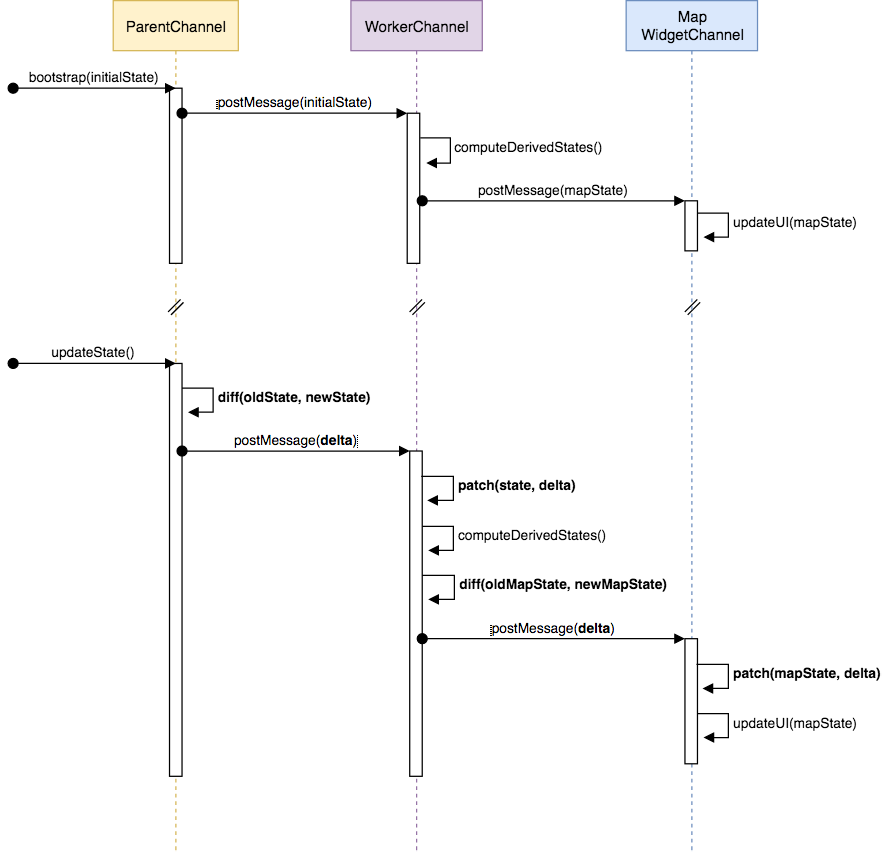
\includegraphics[width=1\columnwidth]{diff-patch} 
  \caption{Sequenza delle chiamate per il flusso diff \& patch}
\end{figure}

Si assicura in tal modo che le dimensioni del carico di trasmissione siano dipendenti unicamente dal numero di modifiche effettuate. Quest'ultime saranno frequenti ma è ragionevole presuporre che ogni modifica statisticamente cambi solo una piccola porzione dello stato applicativo, risultando quindi in piccoli \textit{delta}. \\

\section{Ottimizzazione per immutable state}

Essendo inoltre \textit{Stargate} rivolto verso applicazioni web moderne, in particolare in React \& Redux, l'algoritmo interno di \textit{diff \& patch} assume anche che modifiche allo oggetto stato applicativo non vengano fate per riferimento, ma bensì ritornino una copia avente un nuovo riferimento e le cui proprietà sono anch'esse nuove laddove siano modificate.

\subsection{Strutture dati persistenti}

Una modifica per riferimento è una mutazione diretta ad una struttura dati (un oggetto) esistente senza crearne una copia. Una modifica \textbf{immutable} invece si assicura preventivamente di fare una copia, non profonda, dell'oggetto in qualsiasi caso in cui una proprietà cambi. \\

Ad esempio si assuma di voler modificare la proprietà \texttt{xs.d.g.f} sostituendo 1 con \texttt{{ e: 1 }}. 

\begin{lstlisting}
const xs = {
  d: {
    b: {
      a: 1,
      c: 1
    },
    g: {
      f: 1, // <== da sostituire con { e: 1 }
      h: 1
    }
  }
}
\end{lstlisting}

Modificarlo per riferimento sarebbe eseguire l'istruzione JavaScript \texttt{xs.d.g.f = { e: 1 }}, in quanto viene modificato il campo annidato \texttt{f}, ma sia \texttt{xs} che i suoi sotto-oggetti \texttt{d, g, f} mantengono lo stesso riferimento rispetto a prima.

Una modifica immutabile invece ritorna un nuovo oggetto \texttt{ys}, ove sia \texttt{ys} che i suoi sotto-oggetti \texttt{d', g', f'} hanno nuovi riferimenti mentre \texttt{b} è rimasto invariato poiché non modificato.

\begin{lstlisting}
const ys = {        // <== nuovo riferimento ys
  d: {              // <== nuovo riferimento d
    b: {
      a: 1,
      c: 1
    },
    g: {            // <== nuovo riferimento g
      f: { e: 1 },  // <== nuovo riferimento f
      h: 1
    }
  }
}
\end{lstlisting}

Una possibile rappresentazione della precedente modifica \textit{immutable} è il seguente albero, ove il nuovo oggetto \texttt{ys} possiede sia riferimenti a nuovi oggetti (\texttt{d', g', f'} modificati), che a vecchi (\texttt{b, c, , h} invariati).

\begin{figure}[H] 
  \centering 
  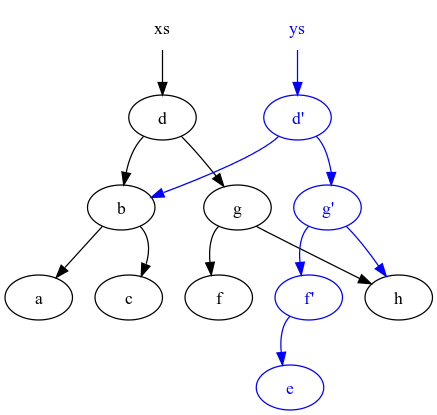
\includegraphics[width=0.5\columnwidth]{immutable} 
  \caption{Albero di \texttt{ys}}
\end{figure}

Strutture dati che preservano sempre la propria precedente versione in caso di modifica si chiamano \textbf{strutture dati persistenti} \footnote{\url{https://en.wikipedia.org/wiki/Persistent_data_structure}} e sono immutabili in quanto le loro operazioni non aggiornano direttamente la struttura, ma bensì generano sempre una nuova aggiornata. 

Tali strutture dati sono fondamentali nei linguaggi di programmazione funzionali, ma nei recenti anni sono divenuti fondamentali anche per linguaggio non puramente funzionali come JavaScript in quanto portano a diversi vantaggi come la diminuizione di \textit{side-effects}.

\subsection{Ottimizzazione dell'algoritmo}

Nel caso specifico dell'algoritmo \textit{diff \& patch}, le strutture immutabili permettono di ottimizzare il calcolo del delta in quanto è sufficiente controllare per riferimento se un campo è cambiato rispetto a prima, senza dover controllare profondamente i valori. Ad esempio confrontando \texttt{xs, ys} dall'esempio precedente, l'algoritmo può evitare di proseguire il calcolo del delta per l'intero sotto-albero \texttt{b} in quanto il riferimento non è cambiato. Se invece viene rilevato un diverso riferimento, l'algoritmo continua lavorando sul sotto-albero. \\

Per uno stato applicativo di notevoli dimensioni, questa ottimizzazione permette di migliorare notevolmente i tempi di \textit{diffing} dell'algoritmo, rendendo il costo linearmente dipendente al numero di modifiche invece che di dimensioni della struttura. Un controllo di riferimento per sapere se un sotto-albero è cambiato ha difatti tempo costante \texttt{O(1)}, altrimenti sarebbe direttamenteproporzionale \texttt{$\Theta$(n)} al numero di campi annidati.
